% Options for packages loaded elsewhere
\PassOptionsToPackage{unicode}{hyperref}
\PassOptionsToPackage{hyphens}{url}
\PassOptionsToPackage{dvipsnames,svgnames,x11names}{xcolor}
%
\documentclass[
]{article}
\usepackage{amsmath,amssymb}
\usepackage{iftex}
\ifPDFTeX
  \usepackage[T1]{fontenc}
  \usepackage[utf8]{inputenc}
  \usepackage{textcomp} % provide euro and other symbols
\else % if luatex or xetex
  \usepackage{unicode-math} % this also loads fontspec
  \defaultfontfeatures{Scale=MatchLowercase}
  \defaultfontfeatures[\rmfamily]{Ligatures=TeX,Scale=1}
\fi
\usepackage{lmodern}
\ifPDFTeX\else
  % xetex/luatex font selection
\fi
% Use upquote if available, for straight quotes in verbatim environments
\IfFileExists{upquote.sty}{\usepackage{upquote}}{}
\IfFileExists{microtype.sty}{% use microtype if available
  \usepackage[]{microtype}
  \UseMicrotypeSet[protrusion]{basicmath} % disable protrusion for tt fonts
}{}
\makeatletter
\@ifundefined{KOMAClassName}{% if non-KOMA class
  \IfFileExists{parskip.sty}{%
    \usepackage{parskip}
  }{% else
    \setlength{\parindent}{0pt}
    \setlength{\parskip}{6pt plus 2pt minus 1pt}}
}{% if KOMA class
  \KOMAoptions{parskip=half}}
\makeatother
\usepackage{xcolor}
\usepackage{longtable,booktabs,array}
\usepackage{calc} % for calculating minipage widths
% Correct order of tables after \paragraph or \subparagraph
\usepackage{etoolbox}
\makeatletter
\patchcmd\longtable{\par}{\if@noskipsec\mbox{}\fi\par}{}{}
\makeatother
% Allow footnotes in longtable head/foot
\IfFileExists{footnotehyper.sty}{\usepackage{footnotehyper}}{\usepackage{footnote}}
\makesavenoteenv{longtable}
\usepackage{graphicx}
\makeatletter
\def\maxwidth{\ifdim\Gin@nat@width>\linewidth\linewidth\else\Gin@nat@width\fi}
\def\maxheight{\ifdim\Gin@nat@height>\textheight\textheight\else\Gin@nat@height\fi}
\makeatother
% Scale images if necessary, so that they will not overflow the page
% margins by default, and it is still possible to overwrite the defaults
% using explicit options in \includegraphics[width, height, ...]{}
\setkeys{Gin}{width=\maxwidth,height=\maxheight,keepaspectratio}
% Set default figure placement to htbp
\makeatletter
\def\fps@figure{htbp}
\makeatother
\setlength{\emergencystretch}{3em} % prevent overfull lines
\providecommand{\tightlist}{%
  \setlength{\itemsep}{0pt}\setlength{\parskip}{0pt}}
\setcounter{secnumdepth}{-\maxdimen} % remove section numbering
\usepackage{preamble_ai_project}
\usepackage[backend=bibtex,style=numeric]{biblatex}
\bibliography{references}
\usepackage{algorithm}
\usepackage{algpseudocode}
\newcommand{\w}{\mathbf{w}}
\newcommand{\x}{\mathbf{x}}
\ifLuaTeX
  \usepackage{selnolig}  % disable illegal ligatures
\fi
\IfFileExists{bookmark.sty}{\usepackage{bookmark}}{\usepackage{hyperref}}
\IfFileExists{xurl.sty}{\usepackage{xurl}}{} % add URL line breaks if available
\urlstyle{same}
\hypersetup{
  colorlinks=true,
  linkcolor={Blue},
  filecolor={Maroon},
  citecolor={Blue},
  urlcolor={Blue},
  pdfcreator={LaTeX via pandoc}}

\author{}
\date{}

\begin{document}

\intro{}

\hypertarget{introduction-rappels-thuxe9oriques}{%
\section{1 -- Introduction \& Rappels
théoriques}\label{introduction-rappels-thuxe9oriques}}

Dans ce document, nous approfondirons des techniques de regression
logistique et ``Naive Bayes'' comme outils d'apprentissage superivisés.

Dans le cadre de l'intelligence artificielle et de l'apprentissage
supervisé, la compréhension et la classification précises des données
revêtent une importance capitale. Parmi les diverses méthodologies
existantes, la Régression Logistique et ``Naive Bayes'' se distinguent
par leur efficacité et leur applicabilité dans de nombreux contextes. Ce
document se propose d'étudier ces deux techniques, en mettant l'accent
sur leur mise en œuvre pratique, et leur efficacité comparative dans
divers scénarios.

\hypertarget{ruxe9gression-logistique}{%
\subsection{1.1 -- Régression
Logistique}\label{ruxe9gression-logistique}}

En statistiques, la régression logistique, s'inscrit dans le cadre des
modèles de régression pour les variables binaires. Bien qu'elle soit
quasiment exclusivement utilisée en tant que méthode de
classification.\\
En effet, c'est l'ajout d'un seuil, à la probabilité continue donnée par
le model de regression qui nous permet de l'utiliser pour la
classification.

Ce type de modèle vise à expliquer de manière optimale une variable
binaire, qui représente la présence ou l'absence d'une caractéristique
spécifique, à l'aide d'un ensemble conséquent de données réelles et d'un
modèle mathématique.

Autrement dit, il s'agit de relier une variable aléatoire de Bernoulli,
généralement notée \(y\), aussi appelé ``label'' à un vecteur constitué
de plusieurs variables aléatoires, \((x_1, \ldots, x_K)\), aussi appelés
``features''. \cite{RegressionLogistique2023}.

La régression logistique s'appuie sur un classifeur linéaire
\cite{ClassifieurLineaire2022} i.e.~un classifieur dont la sortie (pour
un vecteur de feature \(x \in \R^n\)) est donnée par:

\[
g(x) = f(\scalproduct{w}{x} + b)
\] où \(w \in \R^n\) est le vecteur de poids, \(b \in \R\) le biais et
\(\scalproduct{.}{.}\) le produit scalair usuel. \(f\) est une fonction
dite de seuillage qui va séparer nos résultats. Un choix commun pour
\(f\) est la sigmoide ou la fonction signe
\cite{ClassifieurLineaire2022}.

Par exemple, dans le cas de la regression logistique binaire, on suppose
le modèle suivant:

\[
y_i \sim Bernoulli(p_i),\quad p_i = \sigma(\scalproduct{\mathbf{w}}{\mathbf{x}_i} + b),\quad \sigma(z) = \frac{1}{1 + e^{-z}}
\] où \(\mathbf{x}_i \in \R^K\) représente un vecteur (ligne) de \(K\)
valeurs pour les \(K\) features (aussi appelé un \emph{sample}), et
\(y_i\) la variable aléatoire qui représente le label qui leur est
associé.

Cependant, dans notre dataset (voir
\href{#choix-du-dataset-outils-utilisuxe9s}{section 2.0}) nous avons 3
classes (3 espèces d'iris), \(y\) ne suit donc, évidemment, plus une loi
de Bernoulli.\\
La sigmoide étant continue, nous avons simplement modifié la manière
dont nous lui appliquions le seuillage, pour distinguer 3 cas au lieu de
2. i.e.~Au lieu de séparer le domaine en 2
(\(\sigma(z) \leq 0.5,\ \sigma(z) > 0.5\)), nous l'avons séparé en \(N\)
(ici \(N = 3\)). On a donc que
\(y_i = k \Leftrightarrow \frac{k}{N} \leq \sigma(z) < \frac{k + 1}{N}\),
ce qui a donné des résultats plus que satisfaisants comme nous le
verrons en \href{#ruxe9gression-logistique-1}{section 2.2}.

\hypertarget{naive-bayes}{%
\subsection{1.2 -- Naive Bayes}\label{naive-bayes}}

``Naive Bayes'' se présente comme une méthode de classification
probabiliste basée sur le
\href{https://en.wikipedia.org/wiki/Bayes\%27_theorem}{théorème de
Bayes}, caractérisée par l'adoption d'une hypothèse d'indépendance forte
entre les features (attributs), qualifiée de ``naïve''.\\
Plus simplement, le classifieur est classifié de ``naïf'' car il part du
principe que chaque feature (attribut) est indépendante des autres et a
un poid égal quant à la probabilité qu'un point appartienne à une
classe.

Ce model est dit génératif contrairement à la regression logistique
étant considéré comme ``méthode discriminante''
\cite{ClassifieurLineaire2022} et consiste à modéliser les probabilités
conditionnelles \(P(X | classe)\) pour chaque classe \(y\) et vecteur de
features \(X\) afin de trouver celle qui maximise cette probabilité.

En d'autres termes, le problème revient à trouver, pour des attributs
\(X_1, \ldots, X_k\), la classe \(\tilde{y}\) telle que:

\[
\tilde{y} = \text{arg}\max_{Y \in \mathcal{Y}} \left[\  P(Y) \prod_{k = 1}^K{P(X_k | Y)}\  \right]
\]

Citation Test: \cite{LinearModels}

\hypertarget{muxe9thodologie}{%
\section{2 -- Méthodologie}\label{muxe9thodologie}}

\hypertarget{choix-du-dataset-outils-utilisuxe9s}{%
\subsection{2.0 -- Choix du dataset \& outils
utilisés}\label{choix-du-dataset-outils-utilisuxe9s}}

Pour la suite de ce projet les outils suivants ont été utilisés dans
chaque parties:

\begin{itemize}
\tightlist
\item
  \href{https://www.python.org/}{python}
\item
  \href{https://numpy.org/}{numpy}
\item
  \href{https://pandas.pydata.org/}{pandas}
\item
  \href{https://scikit-learn.org/stable/}{sklearn}
\item
  \href{https://matplotlib.org/}{matplotlib}
\item
  \href{https://github.com/uci-ml-repo/ucimlrepo}{ucmilrepo}
\item
  \href{https://docs.pytest.org/en/stable/}{pytest}
\end{itemize}

Le package \texttt{ucmilrepo} a été utilisé pour charger les données de
notre dataset depuis la base de donnée du
\href{https://archive.ics.uci.edu/ml/index}{UC Irvine Machine Learning
Repository}.

Le dataset que nous avons choisi est le fameux dataset ``Iris''
\cite{r.a.fisherIris1936}, un des plus anciens et connus dataset de
classification. Il contient 150 observations de 3 espèces différentes
d'iris (Iris setosa, Iris virginica et Iris versicolor) avec \(K = 4\)
features (longueur et largeur des sépales et pétales).

Voici un aperçu des points-clés du dataset:

\begin{figure}
\centering
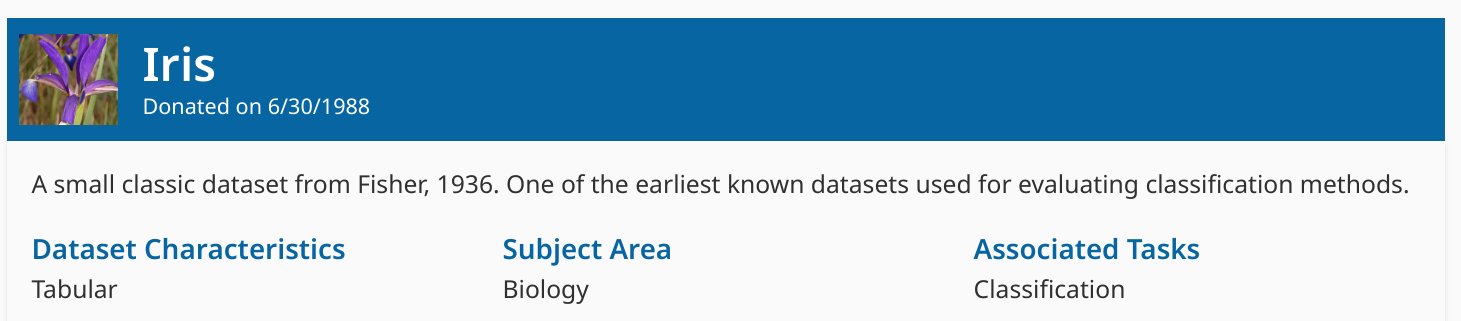
\includegraphics[width=0.8\textwidth,height=\textheight]{../res/iris_img.png}
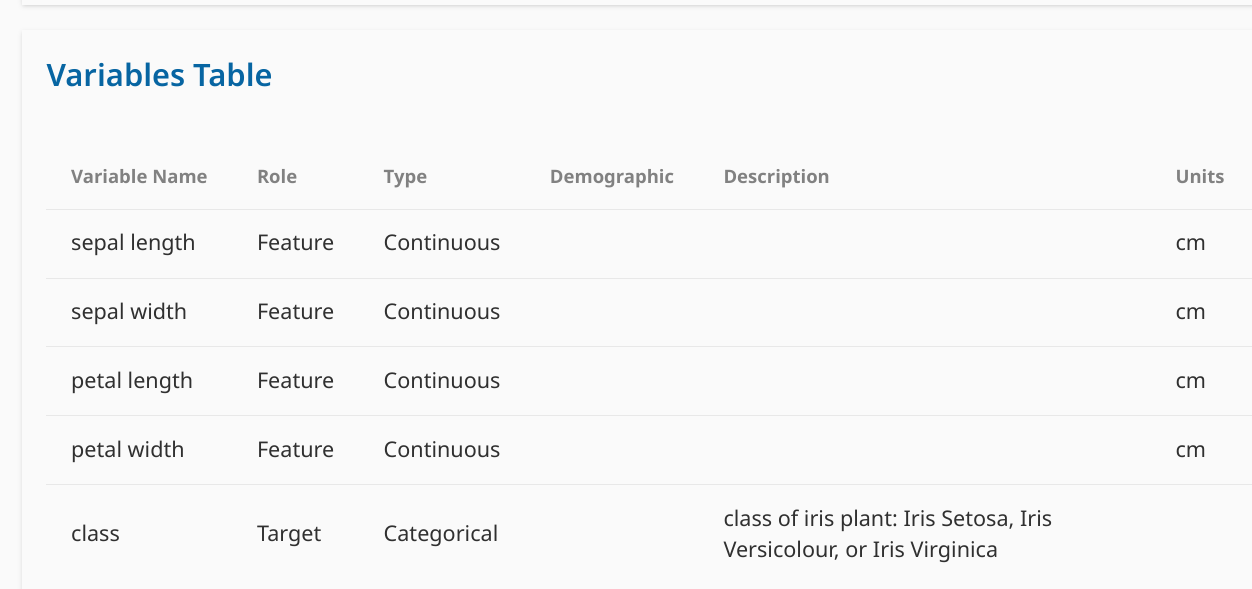
\includegraphics[width=0.8\textwidth,height=\textheight]{../res/iris_table.png}
\caption{Iris descriptive table}
\end{figure}

Le label que nous allons prédire sera donc \emph{class}, i.e.~l'espèce
de l'iris.

\newpage

\hypertarget{gradient-descent}{%
\subsection{2.1 -- Gradient Descent}\label{gradient-descent}}

Dans cette section, une implémentation de la ``descente en gradient'' a
été réalisée. La fonction a la signature suivante

\begin{lstlisting}
  def gradient_descent(df, params: NDArray, alpha: float, num_iters: int) -> NDArray:  
\end{lstlisting}

Elle calcule de manière itérative le(s) paramètre(s) \code{params} qui
minimisent la fonction dont \texttt{df} est le gradient avec un ``taux
de convergence'' \code{alpha}.

La fonction a été testé avec la fonction \code{scipy.optimize.fmin}
\cite{ScipyOptimizeFmin} de la librairie \texttt{scipy} sur la fonction
suivante: \[
f(x) = x * \cos(\pi  (x + 1))
\]

avec différents \(x_0 \in \{-\pi, 0, \pi\}\) (valeur initiale de
\code{params}, i.e.~\texttt{NDArray} avec D=0).

Les minimas locaux trouvés par les deux fonctions sont les suivants:

\begin{figure}
\centering
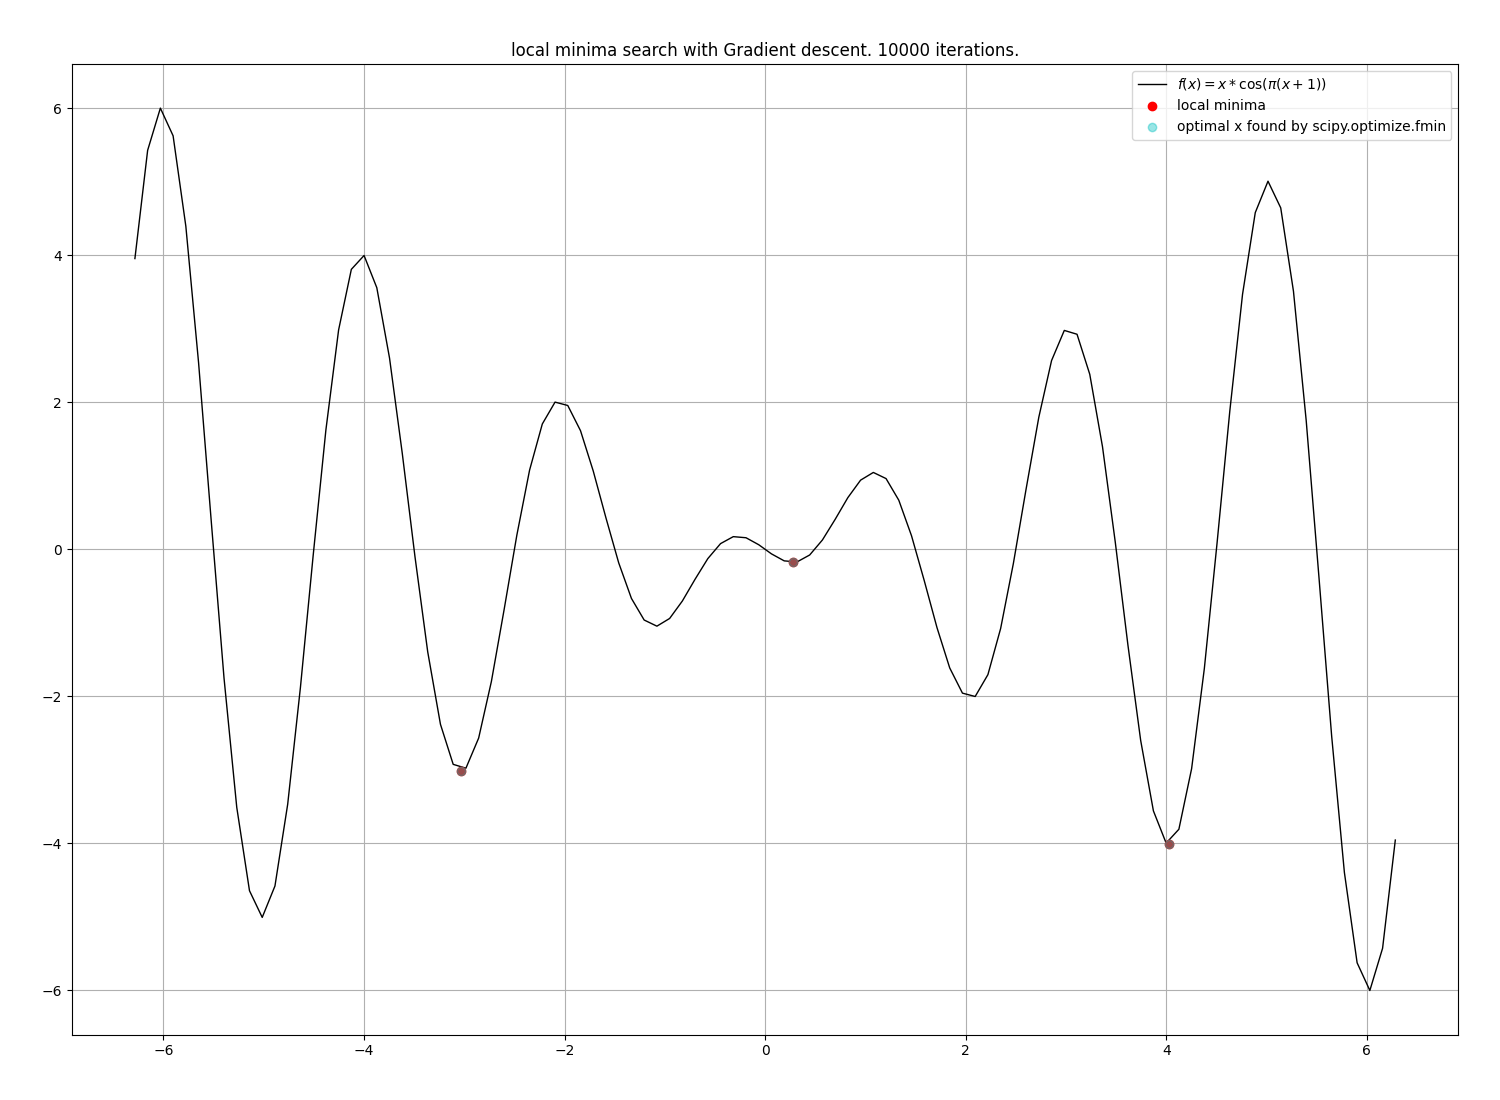
\includegraphics[width=1\textwidth,height=\textheight]{../res/3.1_gradient_descent_minima.png}
\caption{minimas locaux\_gradient descent}
\end{figure}

Ce résultat illustre bien 2 choses: la première est que l'implémentation
de la descente en gradient fonctionne correctement puisque pour chaque
points trouvé par notre fonction est confondu avec celui trouvé par la
fonction de scipy (c'est ce qui donne cette teinte ``grise''). La
deuxième est que la ``qualité'' du minima local (i.e.~la distance avec
le minima globale) dépend fortement de la valeur initiale et ce pour les
deux fonctions.

\newpage{}

\hypertarget{ruxe9gression-logistique-1}{%
\subsection{2.2 -- Régression
Logistique}\label{ruxe9gression-logistique-1}}

\hypertarget{fonction-de-couxfbt-pour-la-ruxe9gression-logistique}{%
\subsubsection{2.2.1 -- Fonction de coût pour la régression
logistique}\label{fonction-de-couxfbt-pour-la-ruxe9gression-logistique}}

\hypertarget{mse-une-mauvaise-iduxe9e}{%
\paragraph{MSE -- Une mauvaise idée}\label{mse-une-mauvaise-iduxe9e}}

:

Afin d'entraîner les paramètres de la régression logistique, il faut
pouvoir comparer les résultats obtenus par la régression avec les
résultats attendus.

Pour cela, on pourrait penser utiliser quelque chose comme la
\texttt{Mean\ Squared\ Error\ (MSE)}, qui est une moyenne du carré de la
différence entre le résultat obtenu par la régression (donné par \(z\))
et la valeur estimée \(y\).

La MSE nous donne une estimation de l'erreur moyenne faite entre la
fonction approximative \(f\) et la valeur attendue \(y\).

L'objectif est donc de minimiser la MSE afin de minimiser l'erreur entre
les valeurs estimées et les valeurs attendues.

Ce qui nous donnerait
\[MSE = \frac{1}{n}\sum_i^n (\sigma(z_i) - y_i)^2\]

avec \(\sigma\) la fonction sigmoïde utilisée pour la régression
logistique, définie comme en section
\href{#ruxe9gression-logistique}{1.1} notre MSE nous donnerait:

\[MSE = \frac{1}{n}\sum_i^n{\left(\frac{1}{1 + e^{-z_i}} - y_i \right)^2}\]

Afin de visualiser la MSE obtenue, nous avons créé un graph de la
fonction \[
\text{MSE}(w, b) = \frac{1}{n} \left( \frac{1}{1+ e^{w^T x + b}} - y_i \right)^2
\] pour \(x = 1\) et \(y = 0.3\). Nous obtenons alors les graphes
suivants:

\begin{longtable}[]{@{}
  >{\centering\arraybackslash}p{(\columnwidth - 2\tabcolsep) * \real{0.5385}}
  >{\centering\arraybackslash}p{(\columnwidth - 2\tabcolsep) * \real{0.4615}}@{}}
\toprule\noalign{}
\begin{minipage}[b]{\linewidth}\centering
Global vision
\end{minipage} & \begin{minipage}[b]{\linewidth}\centering
Zoomed vision
\end{minipage} \\
\midrule\noalign{}
\endhead
\bottomrule\noalign{}
\endlastfoot
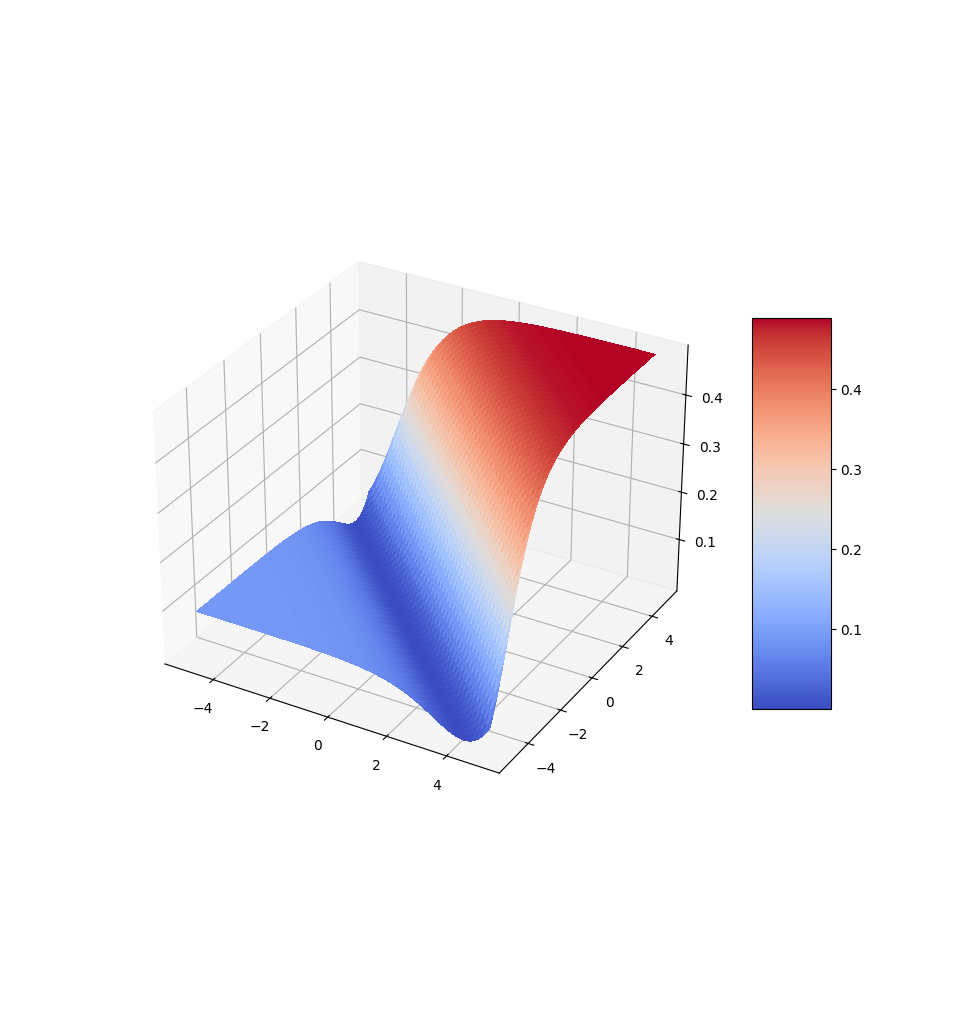
\includegraphics{../res/minima.png} &
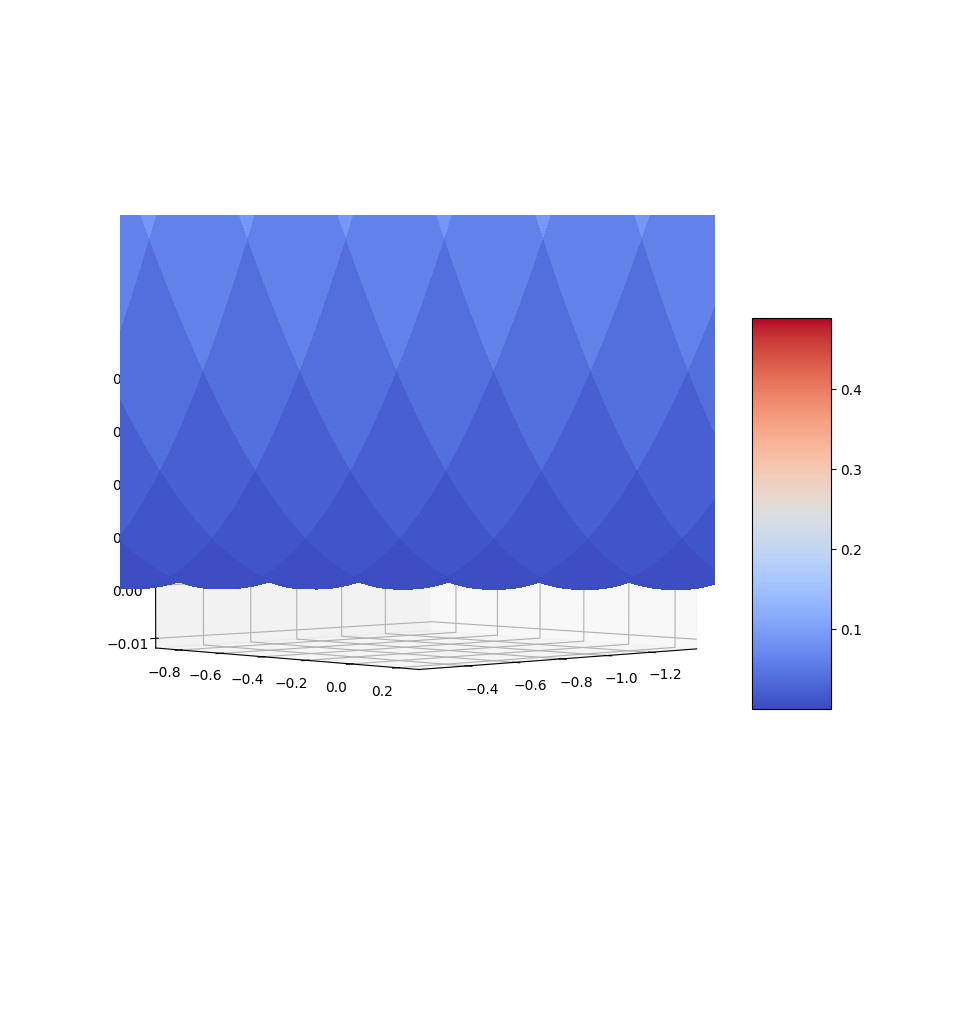
\includegraphics{../res/minima_zoom.png} \\
Fonction MSE avec \(x = 1\) et \(y = 0.3\) (global) & Fonction MSE avec
\(x = 1\) et \(y = 0.3\) (zoomed) \\
\end{longtable}

Nous pouvons remarquer sur la figure zoomé, que la fonction admet
plusieurs minimum locaux. La fonction MSE n'est donc pas convexe. Ceci
est problématique pour la descente en gradient, car celle-ci risquera de
se retrouver coïncé dans un minimum local et ne trouvera jamais le
minimum global.

Si on pouvait faire des plots pour la fonction avec plus de paramètres,
on verrait mieux et plus de minimum locaux.

Cela est dû au fait que la fonction \(\sigma(z)\) n'est pas linéaire.
(Découle trivialement du fait qu'il y ait une exponentielle dans la
fonction.) Ce qui empêche la MSE d'être convexe.

La descente en gradient ne pourra donc pas fonctionnner correctement,
car on pourrait trouver des minimum locaux à la place du minimum global,
ce qui nous empêcherait de trouver les paramètres optimaux pour la
régression logistique.

\hypertarget{log-loss-cross-entropy}{%
\paragraph{Log Loss -- Cross-Entropy}\label{log-loss-cross-entropy}}

:

Pour résoudre ce problème, on utilise plutôt la \texttt{log\ loss}
fonction, appellée également \texttt{cross-entropy}.

La formule de la log loss function est donnée par: \[
C(\mathbf{w},b) = \frac{1}{N} \sum_{i=0}^{N}{ \log p(y_i | \mathbf{x}_i; \mathbf{w}, b) }
\]

avec \(N\) le nombre de sample, \(y_i\) la ``vrai'' classe associé au
sample \(\mathbf{x}_i\) et \(\mathbf{w}, b\) le vecteur de poids et
biais.\\
Où l'on peut ensuite dévolpper \(p(y_i | \mathbf{x}_i; \mathbf{w}, b)\)
pour retomber sur la cross-entropy, avec \(p(x) = y\) et \(q(x) = z\)

La fonction ci-dessus pénalise fortement (du moins plus que les autres
cas) les fausses prédictions ``confiantes'' (i.e.~annonce faux + haute
probabilités) et son domaine d'arrivé est de 0 à \(\infty\), un modèle
parfait aurait une log-loss de 0.\\
Un modèle complètement incorrect aurait, quant à lui, une log loss qui
tend vers \(\infty\)

\hypertarget{apprentissage}{%
\subsubsection{2.2.2 -- Apprentissage}\label{apprentissage}}

Maitenant que nous avons une fonction de coût permettant de quantifier
(en moyenne) à quel point un set de \(N\) prédiction est
correct/incorrect à un point de l'apprentissage donné. Il ne reste plus
qu'à chercher les paramètres optimaux qui minimisent cette fonction de
coût. Ce que l'on va réaliser à l'aide de la descente en gradient. C'est
le processus d'apprentissage.

En effet, lors de l'apprentissage, on va chercher de manière itérative
les \(\mathbf{w}\) et \(b\) qui respectent les critères mentionnés
ci-dessus en calculant le gradient de la fonction de coût à chaque
itérations et en allant dans la direction opposé.

Concrètement cela revient à appliquer l'algorithme suivant:

\begin{algorithm}
\caption{gradient descent}\label{alg:grad_desc}
\begin{algorithmic}
\Function {GradientDescent}{$f, \mathbf{w}_{init}, b_0, \alpha, \text{num\_iters}$}
\State $\mathbf{w}\gets \mathbf{w}_{init}$
\State $b \gets b_0$
\For{1 to num\_iters}
    \State $\mathbf{dw}, db \gets \nabla{f(w, b)} $
    \State $\mathbf{w}\gets \mathbf{w}- \alpha*\mathbf{dw}$
    \State $b \gets b - \alpha*db$
\EndFor
\State \Return $w, b$
\EndFunction
\end{algorithmic}
\end{algorithm}

En pratique, il est plus simple de passer directement la function qui
calcul le gradient en argument, que d'essayer de le calculer
dynamiquement, c'est pourquoi la signature de notre implémentation prend
un \texttt{df} en argument plutôt que la fonction de coût elle même.\\
Où le calcul des dérivées partielles a été definit comme ci-dessous.

Soit
\(\nabla C(\mathbf{w},b) = (\frac{\partial C(\mathbf{w},b)}{\partial \mathbf{w}}, \frac{\partial C(\mathbf{w},b)}{\partial b} )\),
pour un sample \(\mathbf{x}_i\) et sa classe \(y_i\), on obtient:
\begin{align*}
\frac{\partial \log(y_i|\mathbf{x}_i ; \mathbf{w}, b)}{\partial b} 
&= y_i - \sigma(z_i) 
= y_i - \sigma(\mathbf{w}^T X_i + b)\\
%
\frac{\partial \log(y_i|\mathbf{x}_i ; \mathbf{w}, b)}{\partial w_j} 
&= x_{ij}* ( y_i - \sigma(z_i)) 
= (y_i - \sigma(\mathbf{w}^T X_i + b)) * x_{ij}
\end{align*} Or le \texttt{db} dans l'algorithme ci-dessus se refert à
la moyenne (pour tout i) de ces valeurs (i.e.~distance moyenne
\emph{classes prédites} -- \emph{``vrai'' classes}).

On l'obtient donc comme suit: (la somme des dérivées est la dérivée de
la somme, linéarité de la dérivée)
\[\nabla_b\, {C} =\frac{1}{N} \sum_{i = 1}^{N}{ \frac{\partial \log(y_i|\mathbf{x}_i ; \mathbf{w}, b)}{\partial b} =  \frac{1}{N} \sum_{i=1}^N{y_i - \sigma(\mathbf{w}^T X_i + b)}}\]

De même pour \texttt{dw}: \begin{align*}
  \nabla_{\mathbf{w}} C & = \frac{1}{N} \sum_{i = 1}^{N}(x_{ij}(y_i - p_i))_{1 \leq j \leq k} 
  = \frac{1}{N} \sum_{i=1}^N(y_i - \sigma(z_i))\cdot (x_{ij})_{1 \leq j\leq k} \\
%
& =\frac{1}{N}\sum_{i = 1}^N (y_i - \sigma(\mathbf{w}^T\mathbf{x_i} + b))\ \mathbf{x_i}
\end{align*}

On retrouve ainsi, le calcul effectué dans la fonction \code{grad} de
\code{log\_reg.py} de signature suivante:

\begin{lstlisting}
    def grad(X: NDArray, y: NDArray, w: NDArray, b: float) -> tuple:
\end{lstlisting}

Etant donné que pour le calcul du gradient il est nécessaire d'avoir un
matrice de feature \(X\) et vecteur de label \(y\), une version
``modifiée'' de la descente en gradient a été implementé.

\begin{lstlisting}
def grad_desc_ml(features: NDArray, labels: NDArray, df, w: NDArray, b: float, alpha: float, num_iters: int) -> tuple[NDArray, float]:
\end{lstlisting}

Cette fonction se comporte exactement de la même manière que celle
décrite en \href{#gradient-descent}{section 2.1}. La seule différence
est qu'elle passe \texttt{features} et \texttt{labels} comme \texttt{X}
et \texttt{y} à la fonction \texttt{df} (dans notre cas \texttt{df} est
toujours la fonction \texttt{grad}), i.e.~on a
\code{df(features, labels, w, b)} au lieu de \code{df(params)}.

\hypertarget{pruxe9dictions}{%
\subsubsection{2.2.3 -- Prédictions}\label{pruxe9dictions}}

Pour la prédiction, nous avons utilisé la fonction suivante:

\begin{lstlisting}
   def predict_log_reg(X: NDArray, w: NDArray, b):
\end{lstlisting}

qui prend simplement \(\sigma(w^T X + b)\) et seuil la sortie du
sigmoide de manière à retourner un nombre entre 0 et 2 (avec les poids
et bais entraînés).

\newpage{}

\hypertarget{ruxe9sultats}{%
\subsubsection{2.2.4 -- Résultats}\label{ruxe9sultats}}

Suite à l'apprentissage , nous avons obtenu les résultats suivants:
\begin{align*}
    w &= [0.53452349, 0.36463584, 1.16132476, 1.08204578]\\
    b &= 0.45146791
\end{align*}

Nous verrons juste après, le f1-score qu'à généré ces paramètres.

L'apprentissage peut être ré-effectué de manière efficient si besoine
est à l'aide du jupyter notebook
\href{https://github.com/David-Kyrat/13X005-AI-Project/blob/gpu-training/training_test.ipynb}{training\_test.ipynb}
disponible sur la branche
\href{https://github.com/David-Kyrat/13X005-AI-Project/blob/gpu-training/training_test.ipynb}{gpu-training}
du repository github. Le code de l'entraînement (uniquement sur cette
branche) à été ``porté'' sur cuda / gpgpu à l'aide de la librairie
\href{https://cupy.dev}{cupy}.\\
A noter qu'il utilise des fonctions des sklearn alors que nous devions
les implémenter nous mêmes, (telles que les metrics f1-score\ldots). Ces
fonctions ont bien été implenté mais pour une raison de simplicité, elle
n'ont pas été utilisée pour l'entrainement. Le code de cette branche ne
fera donc pas partie du rendu mais reste publiquement accessible sur
github.

\newpage{}

\hypertarget{naive-bayes-1}{%
\subsection{2.3 -- Naive Bayes}\label{naive-bayes-1}}

Dans cette section, une implémentation d'un classifieur linéaire
bayesien (naive bayes) a été réalisée. La fonction de prédictition a la
signature suivante:

\begin{lstlisting}
    #  TODO
\end{lstlisting}

et calcule la classe qui maximise la probabilité conditionnelle définie
en section \href{#naive-bayes}{1.2}.

Dans cette implémentation, étant données que toutes nos features sont
continues, nous avons considéré que \emph{sepal length}, \emph{sepal
width}, \emph{petal length} et \emph{petal width} seront représenté
comme 4 variables aléatoires \(X_0, \cdots, X_3\) suivant 4 lois
normales normales de paramètre \((\mu_k, \sigma_k)\).

C'est à dire: \[
X_k \sim \mathcal{N}( \mu_k, \sigma_k) \qquad \qquad k \in \iitv{0, 3}
\]

\newpage{}

\hypertarget{ruxe9sultats-1}{%
\section{3 -- Résultats}\label{ruxe9sultats-1}}

\printbibliography[heading=bibintoc, title={Références}]

\begin{itemize}
\tightlist
\item
  TODO: ajouter les autres références des documentations utilisées
\end{itemize}

\end{document}
